\documentclass{beamer}
\usetheme{Warsaw}
\usepackage{graphicx}
\usepackage{media9}

\begin{document}

\title{On the Difficulty of Training Recurrent Neural Networks}
\subtitle{Razvan Pascanu, Tomas Mikolov, Yoshua Bengio}


\begin{frame}
	\titlepage
\end{frame}


\begin{frame}
	\frametitle{Overview}
	
	\begin{block}{Contents}
		\begin{itemize}
			\item{Exploding Gradients} 
			\item{Vanishing Gradients} 
			\item{Related Work} 
			\item{Paper Contribution}
			\item{Experimental Results}
		\end{itemize}
	\end{block}
\end{frame}


\begin{frame}
	\frametitle{Exploding Gradients}
	
	\begin{figure}
		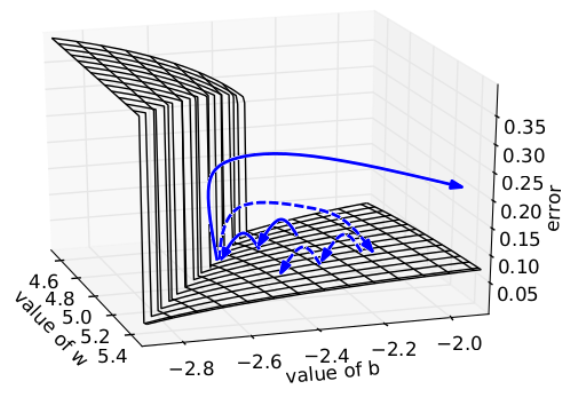
\includegraphics[width=0.8\textwidth]{imgs/geometric_perspective}
	\end{figure}
\end{frame}

\begin{frame}
	\frametitle{Exploding Gradients}
	
	Gradient Descent Method:
	
	\[
		w_{n + 1} = w_{n} - \eta \nabla f(w_{n})
	\]
	
	\begin{itemize}
		\item{$w$: weight}
		\item{$n$: n-th iteration}
		\item{$\eta$: learning rate}
		\item{$f(w)$: cost function}
	\end{itemize}
\end{frame}


\begin{frame}
	\frametitle{Vanishing Gradients}
	
	\begin{figure}
		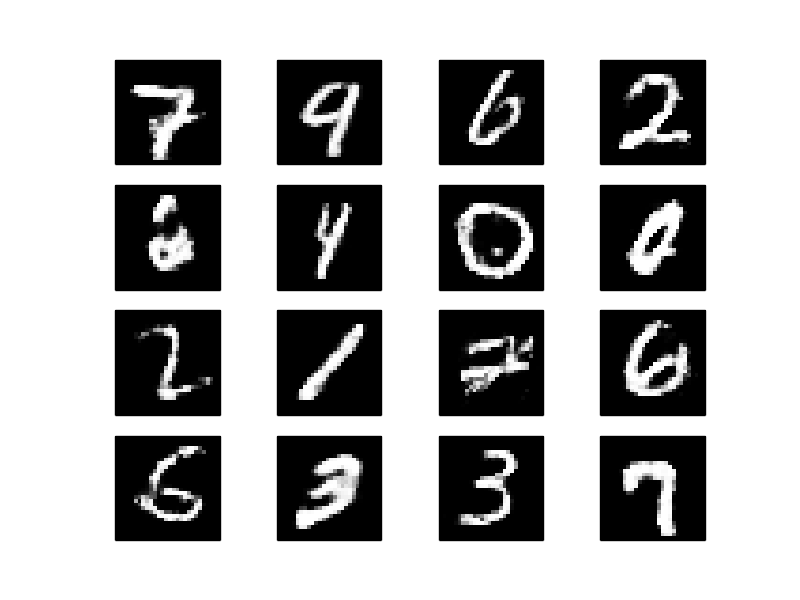
\includegraphics[width=0.8\textwidth]{imgs/mnist}
		\caption{Sample of MNIST dataset}
	\end{figure}
\end{frame}


\begin{frame}
	\frametitle{Vanishing Gradients}
	
	\begin{figure}
		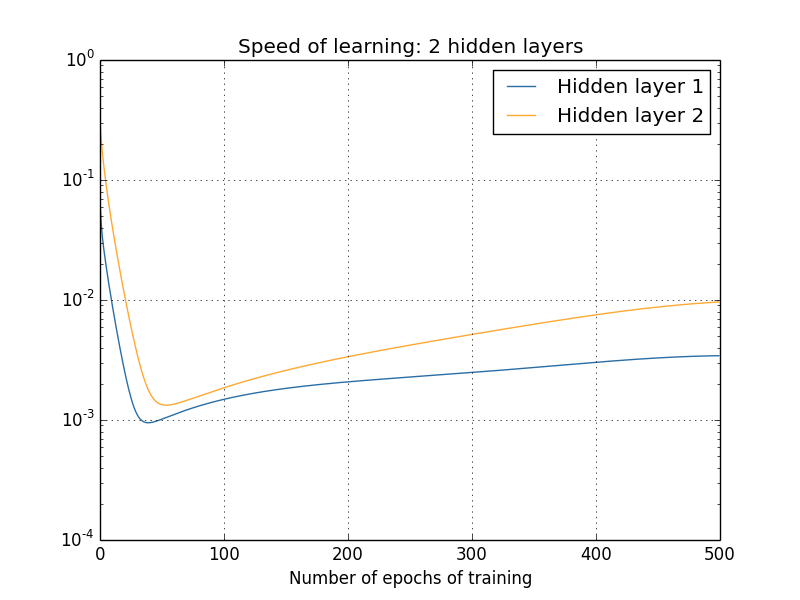
\includegraphics[width=0.8\textwidth]{imgs/training_speed_2_layers}
	\end{figure}
\end{frame}


\begin{frame}
	\frametitle{Vanishing Gradients}
	
	\begin{figure}
		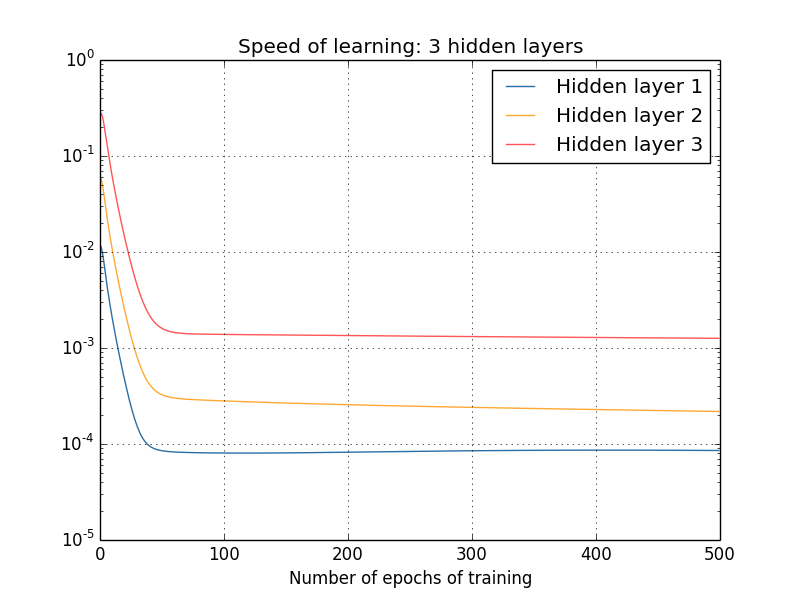
\includegraphics[width=0.8\textwidth]{imgs/training_speed_3_layers}
	\end{figure}
\end{frame}


\begin{frame}
	\frametitle{Vanishing Gradients}
	
	\begin{figure}
		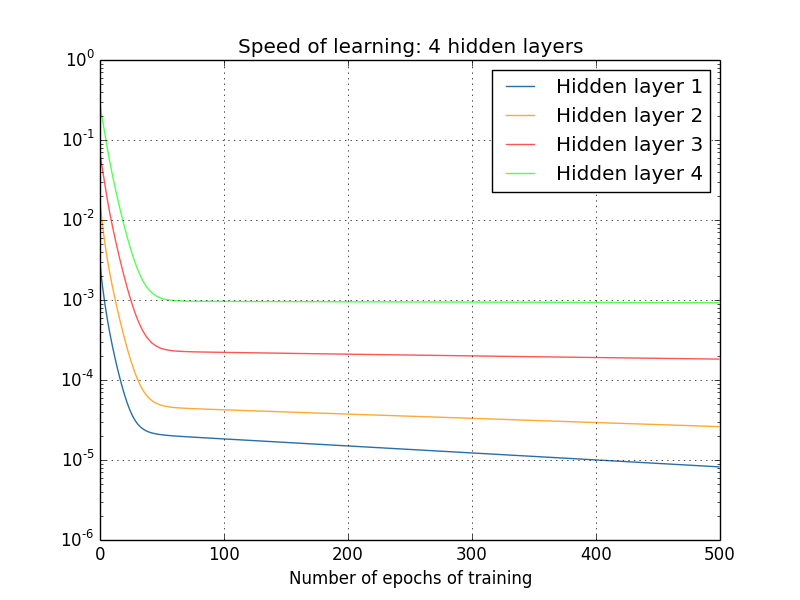
\includegraphics[width=0.8\textwidth]{imgs/training_speed_4_layers}
	\end{figure}
\end{frame}


\begin{frame}
	\frametitle{Vanishing Gradients}
	
	\begin{figure}
		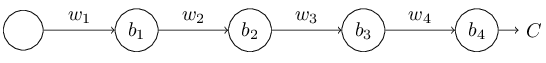
\includegraphics[width=0.8\textwidth]{imgs/chaining}
	\end{figure}
	
		
	\begin{figure}
		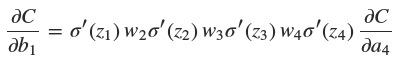
\includegraphics[width=0.8\textwidth]{imgs/chaining_equation}
	\end{figure}
\end{frame}


\begin{frame}
	\frametitle{Vanishing Gradients}
	
	\begin{figure}
		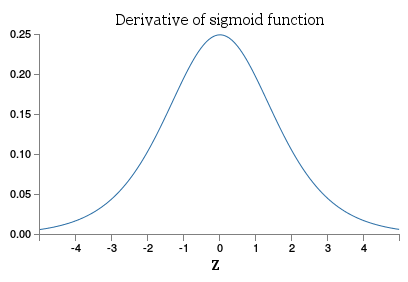
\includegraphics[width=0.8\textwidth]{imgs/sigmoid_derivative}
	\end{figure}
\end{frame}


\begin{frame}
	\frametitle{Vanishing Gradients}
	
	\begin{figure}
		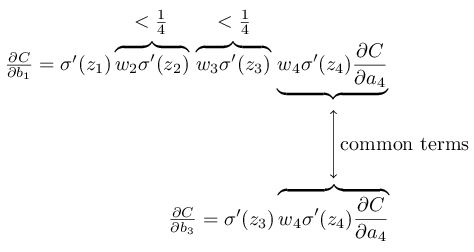
\includegraphics[width=0.8\textwidth]{imgs/chaining_example}
	\end{figure}
\end{frame}


\begin{frame}
	\frametitle{Vanishing Gradients}
	
	\begin{figure}
		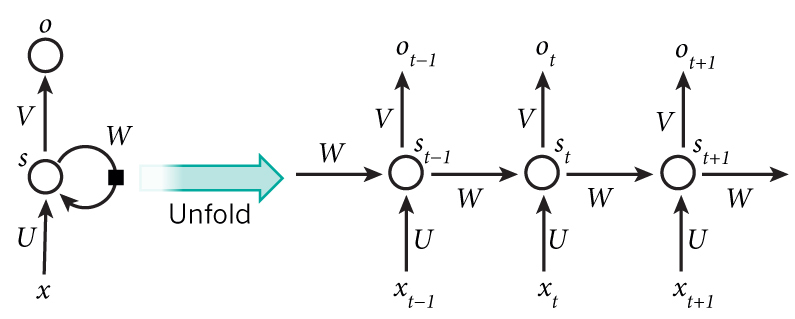
\includegraphics[width=0.8\textwidth]{imgs/rnn_unfolded}
	\end{figure}
\end{frame}


\begin{frame}
	\frametitle{Vanishing Gradients}
	
	\[
		\frac{\partial E}{\partial W} = 
			\sum_{t} \frac{\partial E_{t}}{\partial W}
	\]
	
	\[
		\frac{\partial E_{t}}{\partial W} =
			\frac{\partial E_{t}}{\partial \hat{o_{t}}}
			\frac{\partial \hat{o_{t}}}{\partial s_{t}}
			\frac{\partial s_{t}}{\partial W}
	\]
	
	\[
		\frac{\partial E_{t}}{\partial W} =
			\sum_{k = 0}^{t} 
				\frac{\partial E_{t}}{\partial \hat{o_{t}}}
				\frac{\partial \hat{o_{t}}}{\partial s_{t}}
				\frac{\partial s_{t}}{\partial s_{k}}
				\frac{\partial s_{k}}{\partial W}
	\]
	
	\[
		\frac{\partial E_{t}}{\partial W} =
			\sum_{k = 0}^{t} 
				\frac{\partial E_{t}}{\partial \hat{o_{t}}}
				\frac{\partial \hat{o_{t}}}{\partial s_{t}}
				\left(
					\prod_{j = k + 1}^{t}
						\frac{\partial s_{j}}{\partial s_{j - 1}}
				\right)
				\frac{\partial s_{k}}{\partial W}
	\]
	
\end{frame}



\begin{frame}
	\frametitle{Related Work}
	\begin{block}{Teacher Forcing}
		\begin{itemize}
			\item{Proposed by Doya (1993)}
			\item{Use targets for some or all hidden units to converge towards}
			\item{Assumes model asymptotic behaviour is the same required by the target}
			\item{Requires target to be defined at every time step}
			\item{Reduces exploding gradients}
			\item{Not practical and difficult}
		\end{itemize}
	\end{block}
\end{frame}


\begin{frame}
	\frametitle{Related Work}
	
	\begin{block}{Long Short Term Memory Architecture (LSTM)}
		\begin{itemize}
			\item{Proposed by Hochreiter and Schmidhuber (1997)}
			\item{Introduces Input, Ouput and Forget gates}
			\item{linear unit with self connection of value 1}
			\item{Deals with vanishing but not exploding graidents}
		\end{itemize}
	\end{block}
\end{frame}


\begin{frame}
	\frametitle{Related Work}
	
	\begin{figure}
		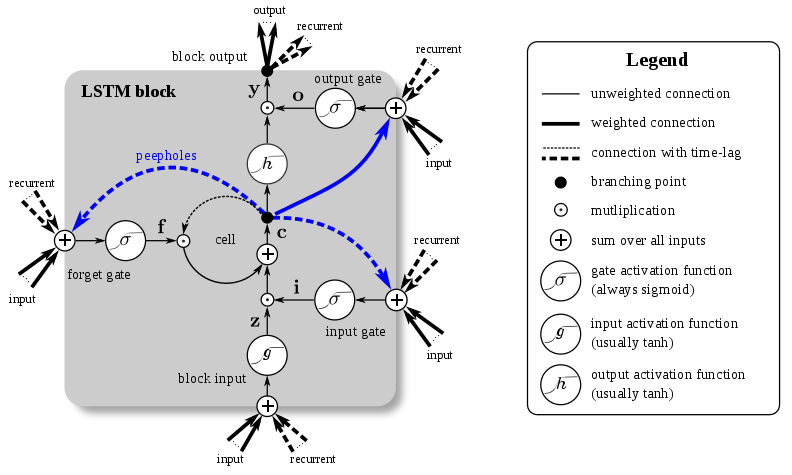
\includegraphics[width=\textwidth]{imgs/LSTM}
	\end{figure}
\end{frame}


\begin{frame}
	\frametitle{Related Work}
	
	\begin{figure}
		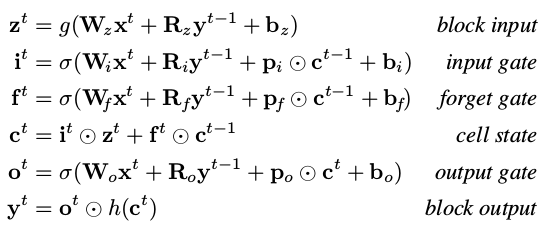
\includegraphics[width=\textwidth]{imgs/LSTM_2}
	\end{figure}
\end{frame}


\begin{frame}
	\frametitle{Related Work}

	\begin{block}{Hessian-Free Optimizer with Structural Damping}
		\begin{itemize}
			\item{Proposed by Sutskever et al (2011)}
		\end{itemize}
		
		\begin{quotation}
			(For Vanishing Problem) ``Presumably this method works because in high dimensional spaces there is a high probability for long term components to be orthogonal to short term ones. This would allow the Hessian  to  rescale  these  components independently."
		\end{quotation}	
	\end{block}
\end{frame}


\begin{frame}
	\frametitle{Related Work}
	
	\begin{block}{Echo State Networks}
		\begin{itemize}
			\item{Proposed by Jaeger and Haas (2014)}
			\item{Avoid exploding and vanishing problem by not learning $W_{rec}$ and $W_{in}$}
			\item{Sparsely connected hidden layer (typically $1\%$)}
			\item{Connectivity and weights are fixed and randomly assigned}
			\item{Only weights of output are learned}
		\end{itemize}
	\end{block}
\end{frame}
	

\begin{frame}
	\frametitle{Scaling Gradient}
	
	\begin{figure}
		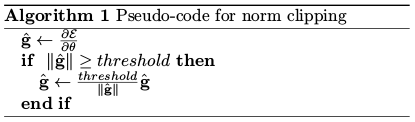
\includegraphics[width=0.8\textwidth]{imgs/gradient_clipping}
	\end{figure}
\end{frame}


\begin{frame}
	\frametitle{Scaling Gradient}
	
	\begin{figure}
		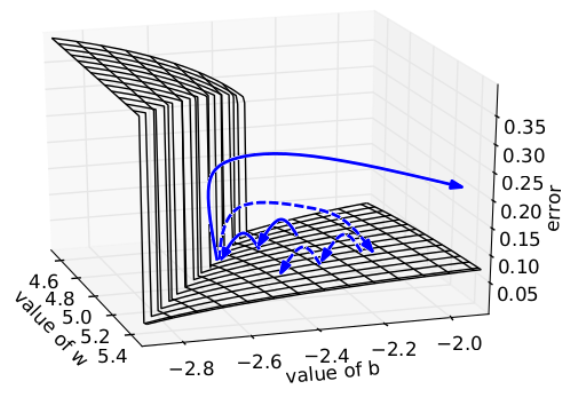
\includegraphics[width=0.8\textwidth]{imgs/geometric_perspective}
	\end{figure}
\end{frame}


\begin{frame}
	\frametitle{Vanishing Gradient Regularizer}
	
	\begin{itemize}
		\item{Vanishing gradients prevents long term latching}
		\item{Increasing the norm $\frac{\partial s_{t}}{\partial s_{k}}$ will increase the sensitivity to all inputs.}
		\item{Creates larger errors}
		\item{In turn causes convergence to suffer}
		\item{Solution is to create a regularizer}
	\end{itemize}
\end{frame}


\begin{frame}
	\frametitle{Vanishing Gradient Regularizer}
	
	\[
		\frac{\partial E_{t}}{\partial W} =
			\sum_{k = 0}^{t} 
			\frac{\partial E_{t}}{\partial \hat{o_{t}}}
			\frac{\partial \hat{o_{t}}}{\partial s_{t}}
			\frac{\partial s_{t}}{\partial s_{k}}
			\frac{\partial s_{k}}{\partial W}
	\]
	
	\[
		\frac{\partial E_{t}}{\partial W} =
			\sum_{k = 0}^{t} 
				\frac{\partial E_{t}}{\partial \hat{o_{t}}}
				\frac{\partial \hat{o_{t}}}{\partial s_{t}}
				\left(
					\prod_{j = k + 1}^{t}
					\frac{\partial s_{j}}{\partial s_{j - 1}}
				\right)
				\frac{\partial s_{k}}{\partial W}
	\]
\end{frame}


\begin{frame}
	\frametitle{Vanishing Gradient Regularizer}
	
	\begin{figure}
		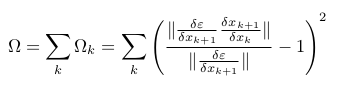
\includegraphics[width=0.8\textwidth]{imgs/vanishing_gradient_regularizer}
	\end{figure}
	
	\begin{itemize}
		\item{Prefers solutions which the error preserves the norm as it travels back in time}
	\end{itemize}
\end{frame}


\begin{frame}
	\frametitle{Experimental Results}
		
	The Temporal Order Problem
	\begin{itemize}
		\item{Long random sequence of discrete symbols}
		\item{\textbf{Beginning} and \textbf{middle} of sequnence will contain one of $\{A, B\}$}
		\item{Task is to classify order of $A, B$}
		\item{Task successful if only $1\%$ of $10,000$ random sequences are misclassified}
	\end{itemize}
	
	
\end{frame}


\begin{frame}
	\frametitle{Experimental Results}	
	\framesubtitle{The Temporal Order Problem}
	Three different RNN intializations were performed for the experiment:
	
	\begin{itemize}
		\item{\textbf{sigmoid unit network}: $W_{rec}, W_{in}, W_{out} \sim \mathcal{N}(0, 0.01)$}
		\item{\textbf{basic tanh unit network}: $W_{rec}, W_{in}, W_{out} \sim \mathcal{N}(0, 0.1)$}		
		\item{\textbf{smart tanh unit network}: $W_{rec}, W_{in}, W_{out} \sim \mathcal{N}(0, 0.01)$} 
	\end{itemize}
	
	Of the three RNN networks three different optimizer configurations were used:
	
	\begin{itemize}
		\item{\textbf{MSGD}: Mini-batch Stochastic Gradient Decent}
		\item{\textbf{MSGD-C}: MSGD with Gradient Clipping}
		\item{\textbf{MSGD-CR}: MSGD-C with Regularization}
	\end{itemize}
\end{frame}


\begin{frame}
	\frametitle{Experimental Results}	
	\framesubtitle{The Temporal Order Problem}
	
	\begin{figure}[H]
		\centering
		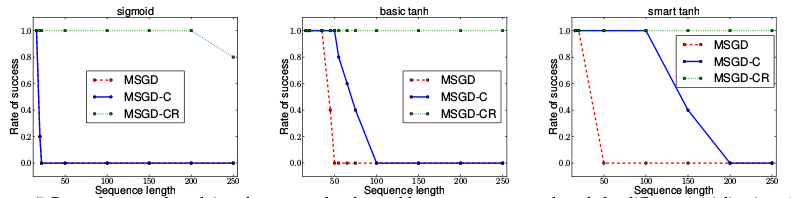
\includegraphics[width=\textwidth]{imgs/experimental_results}
		\label{fig:experimental_results}
	\end{figure}
	
	\begin{itemize}
		\item{5 runs}
		\item{50 hidden unit model}
		\item{Learning rate of 0.01}
		\item{Threshold of 1.0 (for gradient clipping)}
	\end{itemize}	
\end{frame}


\begin{frame}
	\frametitle{Experimental Results}	
	\framesubtitle{Natural Problems}
	
	\begin{figure}[H]
		\centering
		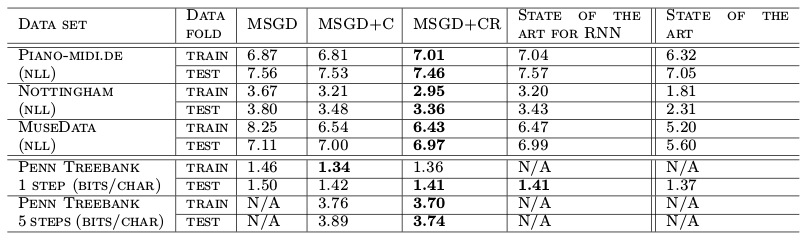
\includegraphics[width=\textwidth]{imgs/experimental_results_2}
		\label{fig:experimental_results}
	\end{figure}
\end{frame}


\begin{frame}
	\centering
	Questions?
\end{frame}


\begin{frame}
	\frametitle{The Genetic Approach}
	
	\begin{figure}[H]
		\centering
		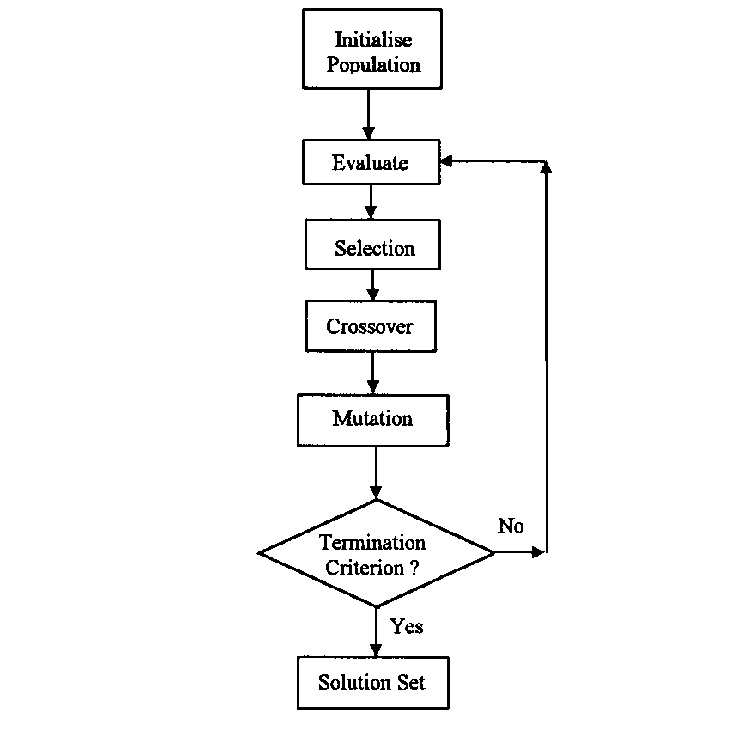
\includegraphics[height=3in]{imgs/ga_algorithm}
		\label{fig:ga_algorithm}
	\end{figure}	
\end{frame}


\begin{frame}
	\frametitle{The Genetic Approach}
	
	\begin{figure}[H]
		\centering
		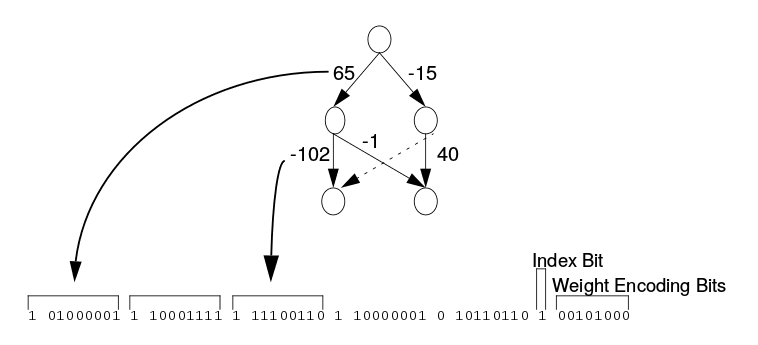
\includegraphics[width=\textwidth]{imgs/genitor_encoding}
		\caption{Whitley's GENITOR Algorithm}
		\label{fig:ga_algorithm}
	\end{figure}	
\end{frame}


\begin{frame}
	\frametitle{The Genetic Approach}
	
	\begin{figure}[H]
		\centering
		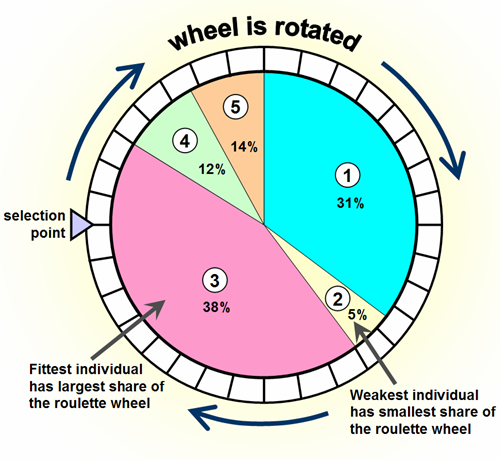
\includegraphics[width=0.6\textwidth]{imgs/fitness_proportionate_selection}
		\caption{Fitness Proportionate Selection}
		\label{fig:ga_algorithm}
	\end{figure}	
\end{frame}


\begin{frame}
	\frametitle{The Genetic Approach}
	
	\begin{figure}[H]
		\centering
		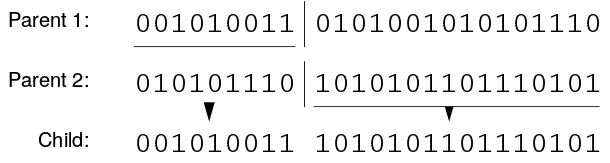
\includegraphics[width=\textwidth]{imgs/point_crossover}
		\caption{Point Crossover}
		\label{fig:ga_algorithm}
	\end{figure}	
\end{frame}


\begin{frame}
	\frametitle{The Genetic Approach}
	Example Applications:
	
	\begin{itemize}
		\item{MarI/O (NEAT Algorithm): Plays a level of Mario \href{https://www.youtube.com/watch?v=qv6UVOQ0F44}{\beamergotobutton{YouTube}}}
		
		\item{Evolving Gaits for Legged Robots (HyperNEAT) \href{https://www.youtube.com/watch?v=V2ADU8YWIug}{\beamergotobutton{YouTube}}}
	\end{itemize}
\end{frame}
\end{document}